%!TEX root = ceres-solver.tex
\chapter{Fitting a Curve to Data}
\label{chapter:tutorial:curvefitting}
The examples we have seen until now are simple optimization problems with no data. The original purpose of least squares and non-linear least squares analysis was fitting curves to data. It is only appropriate that we now consider an example of such a problem\footnote{The full code and data for this example can be found in
\texttt{examples/data\_fitting.cc}. It contains data generated by sampling the curve $y = e^{0.3x + 0.1}$ and adding Gaussian noise with standard deviation $\sigma = 0.2$.}. Let us fit some data to the curve
\begin{equation}
	y = e^{mx + c}.
\end{equation}

We begin by defining a templated object to evaluate the residual. There will be a residual for each observation.
\begin{minted}[mathescape]{c++}
class ExponentialResidual {
 public:
  ExponentialResidual(double x, double y)
      : x_(x), y_(y) {}

  template <typename T> bool operator()(const T* const m,
                                        const T* const c,
                                        T* residual) const {
    // $y - e^{mx + c}$
    residual[0] = T(y_) - exp(m[0] * T(x_) + c[0]);  
    return true;
  }

 private:
  // Observations for a sample.
  const double x_;
  const double y_;
};
\end{minted}
%\caption{Templated functor to compute the residual for the exponential model fitting problem. Note that one instance of the functor is responsible for computing the residual for one observation.}
%\label{listing:exponentialresidual}
%\end{listing}
Assuming the observations are in a $2n$ sized array called \texttt{data}, the problem construction is a simple matter of creating a \texttt{CostFunction} for every observation.
\clearpage
\begin{minted}{c++}
double m = 0.0;
double c = 0.0;

Problem problem;
for (int i = 0; i < kNumObservations; ++i) {
  problem.AddResidualBlock(
      new AutoDiffCostFunction<ExponentialResidual, 1, 1, 1>(
          new ExponentialResidual(data[2 * i], data[2 * i + 1])),
      NULL,
      &m, &c);
}
\end{minted}
Compiling and running \texttt{data\_fitting.cc} gives us
\begin{minted}{bash}
 0: f: 1.211734e+02 d: 0.00e+00 g: 3.61e+02 h: 0.00e+00 rho: 0.00e+00 mu: 1.00e-04 li:  0
 1: f: 1.211734e+02 d:-2.21e+03 g: 3.61e+02 h: 7.52e-01 rho:-1.87e+01 mu: 2.00e-04 li:  1
 2: f: 1.211734e+02 d:-2.21e+03 g: 3.61e+02 h: 7.51e-01 rho:-1.86e+01 mu: 8.00e-04 li:  1
 3: f: 1.211734e+02 d:-2.19e+03 g: 3.61e+02 h: 7.48e-01 rho:-1.85e+01 mu: 6.40e-03 li:  1
 4: f: 1.211734e+02 d:-2.02e+03 g: 3.61e+02 h: 7.22e-01 rho:-1.70e+01 mu: 1.02e-01 li:  1
 5: f: 1.211734e+02 d:-7.34e+02 g: 3.61e+02 h: 5.78e-01 rho:-6.32e+00 mu: 3.28e+00 li:  1
 6: f: 3.306595e+01 d: 8.81e+01 g: 4.10e+02 h: 3.18e-01 rho: 1.37e+00 mu: 1.09e+00 li:  1
 7: f: 6.426770e+00 d: 2.66e+01 g: 1.81e+02 h: 1.29e-01 rho: 1.10e+00 mu: 3.64e-01 li:  1
 8: f: 3.344546e+00 d: 3.08e+00 g: 5.51e+01 h: 3.05e-02 rho: 1.03e+00 mu: 1.21e-01 li:  1
 9: f: 1.987485e+00 d: 1.36e+00 g: 2.33e+01 h: 8.87e-02 rho: 9.94e-01 mu: 4.05e-02 li:  1
10: f: 1.211585e+00 d: 7.76e-01 g: 8.22e+00 h: 1.05e-01 rho: 9.89e-01 mu: 1.35e-02 li:  1
11: f: 1.063265e+00 d: 1.48e-01 g: 1.44e+00 h: 6.06e-02 rho: 9.97e-01 mu: 4.49e-03 li:  1
12: f: 1.056795e+00 d: 6.47e-03 g: 1.18e-01 h: 1.47e-02 rho: 1.00e+00 mu: 1.50e-03 li:  1
13: f: 1.056751e+00 d: 4.39e-05 g: 3.79e-03 h: 1.28e-03 rho: 1.00e+00 mu: 4.99e-04 li:  1
Ceres Solver Report: Iterations: 13, Initial cost: 1.211734e+02, \
Final cost: 1.056751e+00, Termination: FUNCTION_TOLERANCE.
Initial m: 0 c: 0
Final   m: 0.291861 c: 0.131439
\end{minted}

\begin{figure}[t]
	\begin{center}
	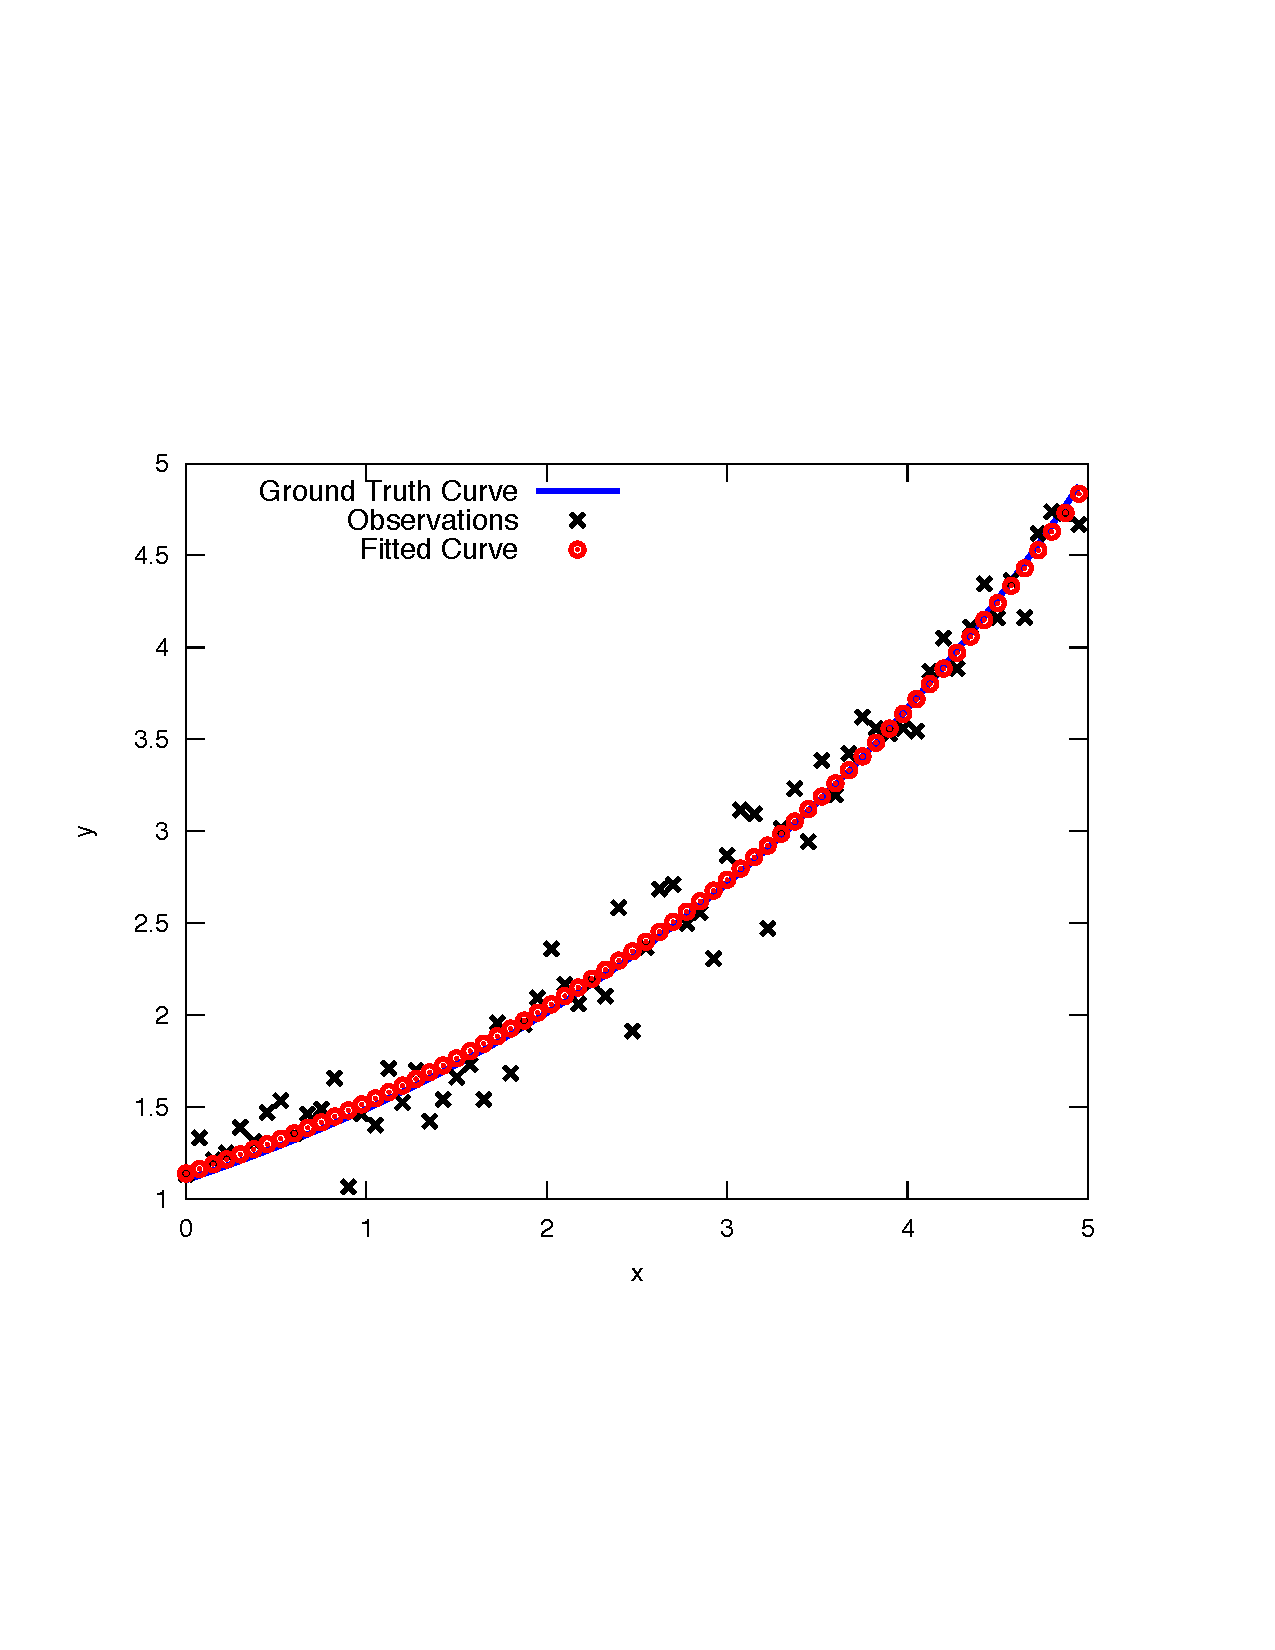
\includegraphics[width=\textwidth]{fit.pdf}
	\caption{Least squares data fitting to the curve $y = e^{0.3x + 0.1}$. Observations were generated by sampling this curve uniformly in the interval $x=(0,5)$ and adding Gaussian noise with $\sigma = 0.2$.\label{fig:exponential}}
\end{center}
\end{figure}

Starting from parameter values $m = 0, c=0$ with an initial objective function value of $121.173$ Ceres finds a solution $m= 0.291861, c = 0.131439$ with an objective function value of $1.05675$. These values are a a bit different than the parameters of the original model $m=0.3, c= 0.1$, but this is expected. When reconstructing a curve from noisy data, we expect to see such deviations. Indeed, if you were to evaluate the objective function for $m=0.3, c=0.1$, the fit is worse with an objective function value of 1.082425. Figure~\ref{fig:exponential} illustrates the fit.
